% !TEX program = xelatex
\documentclass[12pt,a4paper]{article}

\usepackage{fontspec}
\usepackage{polyglossia}
\setmainlanguage{greek}
\setotherlanguage{english}
\setmainfont[Script=Greek]{DejaVu Serif}
\setsansfont[Script=Greek]{DejaVu Sans}
\setmonofont[Script=Greek]{DejaVu Sans Mono}
\newfontfamily\greekfonttt[Script=Greek]{DejaVu Sans Mono}

\usepackage[a4paper, margin=2.45cm]{geometry}
\usepackage{amsmath, amssymb}
\usepackage{booktabs}
\usepackage{array}
\usepackage{graphicx}
\usepackage{float}
\usepackage{caption}
\usepackage[hidelinks]{hyperref}
\usepackage{enumitem}
\usepackage{parskip}
\usepackage{xcolor}
\usepackage{listings}
\usepackage{fancyhdr}

\pagestyle{fancy}
\fancyhf{}
\lhead{4η Εργασία -- Explanatory Report}
\rhead{Ερώτημα 3}
\cfoot{\thepage}
\setlength{\headheight}{14.5pt}

\newcommand{\code}[1]{\texttt{\textenglish{#1}}}

\lstset{
    basicstyle=\ttfamily\small,
    breaklines=true,
    frame=single,
    backgroundcolor=\color{gray!8},
    columns=fullflexible,
    keepspaces=true
}

\title{
    \textbf{Ανάλυση Δεδομένων 2025--26}\\[0.25cm]
    \Large 4η Εργασία -- Explanatory Report\\[0.15cm]
    \large Ερώτημα 3: Random Forest με 200 εκτιμητές και $m=p/2$
}
\author{
    Ρακοβαλής Παύλος\\
    ΑΕΜ: 6931
}
\date{\today}

\begin{document}

\maketitle
\thispagestyle{fancy}

\begin{abstract}
Το παρόν κείμενο εξηγεί αναλυτικά το τρίτο ερώτημα της 4ης εργασίας, στο
οποίο εφαρμόζεται η μέθοδος Random Forest για την πρόβλεψη του τύπου κρασιού.
Το report είναι γραμμένο με εκπαιδευτικό ύφος, σαν να απευθύνεται σε αναγνώστη
που τώρα μαθαίνει Ανάλυση Δεδομένων. Πρώτα εξηγείται τι ζητάει το ερώτημα,
έπειτα παρουσιάζεται η θεωρία πίσω από το Random Forest και τέλος περιγράφεται
βήμα προς βήμα η υλοποίηση. Το Random Forest με 200 δέντρα και
\code{max\_features=5} πέτυχε test accuracy 0.9666.
\end{abstract}

\tableofcontents
\newpage

%=============================================================================
\section{Το ερώτημα της εργασίας}
%=============================================================================

Το τρίτο ερώτημα της 4ης εργασίας είναι:

\begin{quote}
\textbf{«Να γίνει πρόβλεψη/εκτίμηση του τύπου κρασιού με τη μέθοδο Random
Forest, χρησιμοποιώντας εκτιμήσεις από 200 δειγματοληψίες
(\code{n\_estimators=200}) και τυχαίο πλήθος υποψήφιων χαρακτηριστικών
$m=p/2$, όπου $p$ είναι το σύνολο των χαρακτηριστικών του προβλήματος.»}
\end{quote}

Με απλά λόγια, η εργασία ζητά να προβλέψουμε ξανά αν ένα κρασί είναι λευκό ή
κόκκινο, αλλά αυτή τη φορά με τη μέθοδο \textbf{Random Forest}.

Το Random Forest μοιάζει πολύ με το Bagging του προηγούμενου ερωτήματος, επειδή
και αυτό χρησιμοποιεί πολλά δέντρα ταξινόμησης. Όμως έχει μία επιπλέον ιδέα:
όταν κάθε δέντρο κάνει έναν διαχωρισμό, δεν εξετάζει όλες τις διαθέσιμες
μεταβλητές. Εξετάζει μόνο ένα τυχαίο υποσύνολο μεταβλητών.

Στο συγκεκριμένο ερώτημα ζητείται:

\begin{center}
\code{n\_estimators = 200}
\end{center}

δηλαδή 200 δέντρα, και:

\[
    m = \frac{p}{2},
\]

όπου $p$ είναι το πλήθος των predictors.

\subsection{Τι πρέπει να κάνουμε πρακτικά}

Για να λύσουμε το ερώτημα, πρέπει να κάνουμε τα εξής:

\begin{enumerate}[label=\arabic*.]
    \item Να χρησιμοποιήσουμε τα δεδομένα της 3ης εργασίας.
    \item Να προβλέψουμε τη μεταβλητή \code{wine\_type}.
    \item Να μη χρησιμοποιήσουμε τη μεταβλητή \code{quality}.
    \item Να κρατήσουμε το ίδιο training/test split: 70\% και 30\%.
    \item Να εφαρμόσουμε Random Forest με 200 δέντρα.
    \item Να ορίσουμε το πλήθος υποψήφιων χαρακτηριστικών ανά split ίσο με
    $m=p/2$.
    \item Να υπολογίσουμε την test accuracy.
    \item Να παρουσιάσουμε και να εξηγήσουμε τον confusion matrix.
\end{enumerate}

%=============================================================================
\section{Υπενθύμιση του προβλήματος}
%=============================================================================

Το πρόβλημα παραμένει το ίδιο με τα δύο προηγούμενα ερωτήματα. Έχουμε
παρατηρήσεις κρασιών και θέλουμε να προβλέψουμε τον τύπο του κρασιού:

\begin{center}
\code{red} ή \code{white}.
\end{center}

Η μεταβλητή στόχος είναι:

\begin{center}
\code{wine\_type}.
\end{center}

Η κωδικοποίηση είναι:

\begin{center}
\code{red = 0} \hspace{1cm} και \hspace{1cm} \code{white = 1}.
\end{center}

Οι προβλεπτικές μεταβλητές είναι όλες οι φυσικοχημικές μεταβλητές εκτός από τη
\code{quality}. Συνολικά χρησιμοποιούνται:

\[
    p = 11
\]

προβλεπτικές μεταβλητές.

\begin{center}
\footnotesize
\begin{tabular}{lll}
\toprule
\code{fixed acidity} & \code{volatile acidity} & \code{citric acid} \\
\code{residual sugar} & \code{chlorides} & \code{free sulfur dioxide} \\
\code{total sulfur dioxide} & \code{density} & \code{pH} \\
\code{sulphates} & \code{alcohol} & \\
\bottomrule
\end{tabular}
\end{center}

Το training/test split ήταν:

\begin{center}
\begin{tabular}{lrr}
\toprule
\textbf{Σύνολο} & \textbf{Πλήθος} & \textbf{Ποσοστό} \\
\midrule
Training set & 3706 & 70\% \\
Test set & 1589 & 30\% \\
\bottomrule
\end{tabular}
\end{center}

Χρησιμοποιήθηκε και πάλι:

\begin{center}
\code{random\_state = 6931}
\end{center}

ώστε τα αποτελέσματα να είναι αναπαραγώγιμα και συγκρίσιμα με τα προηγούμενα
ερωτήματα.

%=============================================================================
\section{Θεωρητικό υπόβαθρο: από Bagging σε Random Forest}
%=============================================================================

Στο Ερώτημα 2 είδαμε τη μέθοδο Bagging. Το Bagging εκπαιδεύει πολλά δέντρα σε
διαφορετικά bootstrap δείγματα και στο τέλος συνδυάζει τις προβλέψεις τους με
πλειοψηφική ψηφοφορία.

Το Random Forest κρατά αυτή τη βασική ιδέα, αλλά προσθέτει ένα ακόμη επίπεδο
τυχαιότητας.

\subsection{Η βασική ιδέα του Random Forest}

Το Random Forest είναι ένα «δάσος» από πολλά δέντρα ταξινόμησης. Κάθε δέντρο
εκπαιδεύεται σε ένα διαφορετικό bootstrap δείγμα, όπως στο Bagging.

Η επιπλέον διαφορά είναι η εξής:

\begin{quote}
Σε κάθε split κάθε δέντρου, το μοντέλο δεν εξετάζει όλες τις μεταβλητές.
Εξετάζει μόνο ένα τυχαίο υποσύνολο μεταβλητών.
\end{quote}

Αυτό σημαίνει ότι τα δέντρα γίνονται πιο διαφορετικά μεταξύ τους. Και αυτό
είναι πολύ χρήσιμο σε ένα ensemble μοντέλο.

\subsection{Γιατί θέλουμε τα δέντρα να είναι διαφορετικά}

Αν όλα τα δέντρα ενός ensemble είναι σχεδόν ίδια, τότε θα κάνουν περίπου τα
ίδια λάθη. Σε αυτή την περίπτωση, η ψηφοφορία πολλών δέντρων δεν βοηθά τόσο
πολύ, γιατί όλα τα δέντρα συμφωνούν για τους ίδιους λόγους.

Αν όμως τα δέντρα είναι διαφορετικά μεταξύ τους, τότε το ένα μπορεί να
διορθώνει τα λάθη του άλλου. Έτσι, η τελική απόφαση της πλειοψηφίας γίνεται
πιο σταθερή.

Το Random Forest προσπαθεί να δημιουργήσει αυτή τη διαφορετικότητα με δύο
τρόπους:

\begin{enumerate}[label=\arabic*.]
    \item Κάθε δέντρο εκπαιδεύεται σε διαφορετικό bootstrap δείγμα.
    \item Σε κάθε split εξετάζεται τυχαίο υποσύνολο χαρακτηριστικών.
\end{enumerate}

\subsection{Διαφορά Bagging και Random Forest}

Η βασική διαφορά είναι:

\begin{center}
\begin{tabular}{p{5cm}p{7cm}}
\toprule
\textbf{Bagging} & \textbf{Random Forest} \\
\midrule
Πολλά δέντρα σε bootstrap δείγματα. &
Πολλά δέντρα σε bootstrap δείγματα. \\
\addlinespace
Σε κάθε split κάθε δέντρο μπορεί να εξετάσει όλες τις μεταβλητές. &
Σε κάθε split κάθε δέντρο εξετάζει μόνο τυχαίο υποσύνολο μεταβλητών. \\
\addlinespace
Τα δέντρα μπορεί να μοιάζουν αρκετά μεταξύ τους, ειδικά αν υπάρχουν πολύ ισχυροί predictors. &
Τα δέντρα αναγκάζονται να είναι πιο διαφορετικά μεταξύ τους. \\
\bottomrule
\end{tabular}
\end{center}

Άρα το Random Forest είναι σαν Bagging, αλλά με επιπλέον τυχαιότητα στην
επιλογή των μεταβλητών.

\begin{figure}[H]
\centering
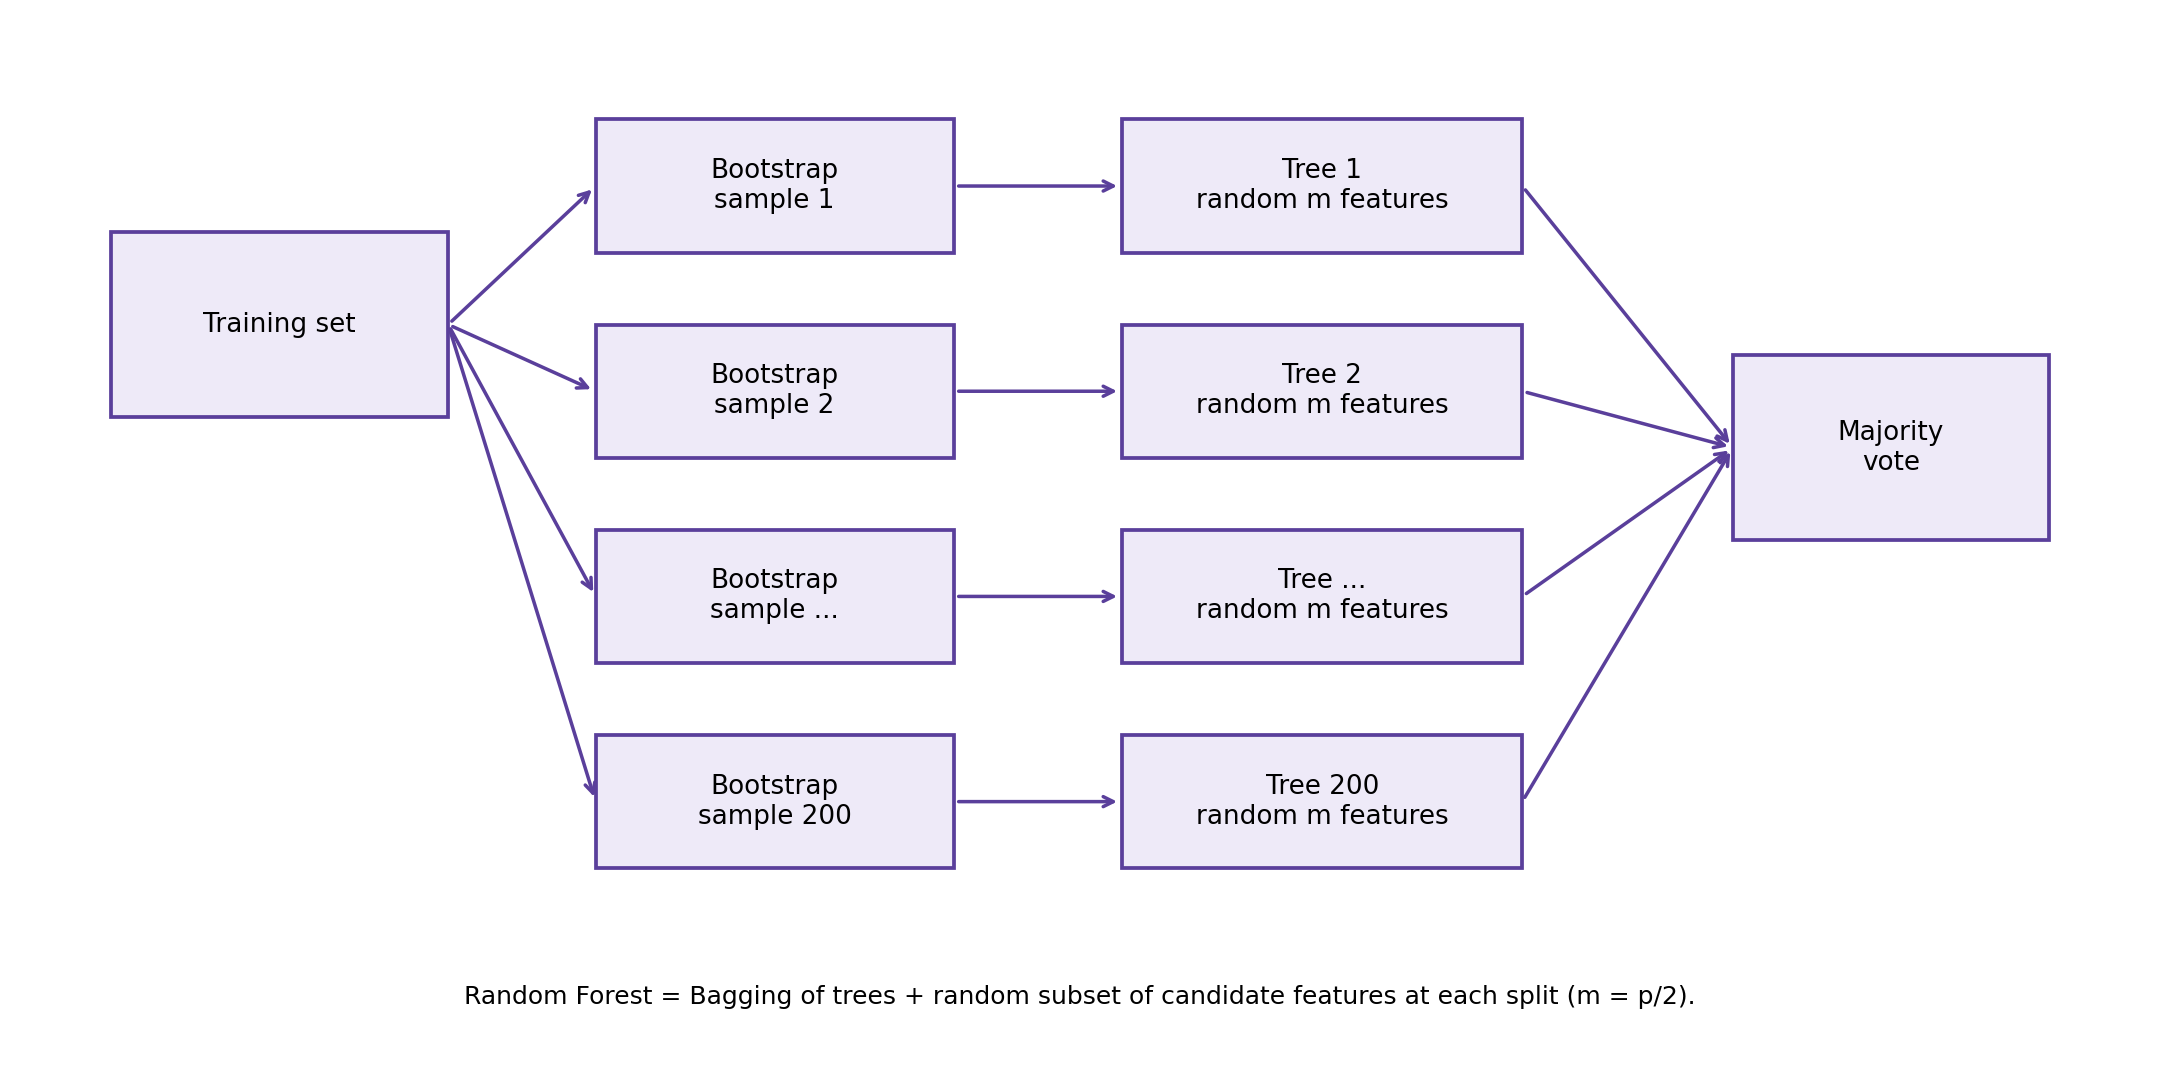
\includegraphics[width=0.92\textwidth]{q3_random_forest_concept.png}
\caption{Η βασική ιδέα του Random Forest: bootstrap δείγματα, τυχαία χαρακτηριστικά ανά split και τελική ψηφοφορία.}
\end{figure}

%=============================================================================
\section{Τι σημαίνει $m=p/2$}
%=============================================================================

Η εκφώνηση ζητά το τυχαίο πλήθος υποψήφιων χαρακτηριστικών να είναι:

\[
    m = \frac{p}{2}.
\]

Εδώ:

\begin{itemize}
    \item $p$ είναι το συνολικό πλήθος προβλεπτικών μεταβλητών.
    \item $m$ είναι πόσες από αυτές θα εξετάζονται ως υποψήφιες σε κάθε split.
\end{itemize}

Στη δική μας περίπτωση:

\[
    p = 11.
\]

Άρα:

\[
    \frac{p}{2} = \frac{11}{2} = 5.5.
\]

Όμως το \code{scikit-learn}, όταν δίνουμε το \code{max\_features} ως ακέραιο
πλήθος μεταβλητών, χρειάζεται ακέραιο αριθμό. Δεν μπορούμε να του πούμε να
εξετάζει 5.5 μεταβλητές. Για τον λόγο αυτό χρησιμοποιήθηκε:

\begin{center}
\code{max\_features = 5}.
\end{center}

Με άλλα λόγια, σε κάθε split κάθε δέντρου, το Random Forest εξετάζει τυχαία 5
από τις 11 διαθέσιμες προβλεπτικές μεταβλητές.

\subsection{Γιατί δεν εξετάζουμε όλες τις μεταβλητές}

Αν εξετάζαμε όλες τις μεταβλητές σε κάθε split, το Random Forest θα έμοιαζε
πολύ περισσότερο με Bagging. Τα δέντρα θα είχαν μεγαλύτερη πιθανότητα να
χρησιμοποιούν ξανά και ξανά τις ίδιες ισχυρές μεταβλητές.

Με το \code{max\_features=5}, κάθε split βλέπει μόνο μέρος των μεταβλητών.
Αυτό αναγκάζει τα δέντρα να δοκιμάσουν διαφορετικούς συνδυασμούς μεταβλητών.
Έτσι μειώνεται η ομοιότητα μεταξύ των δέντρων.

%=============================================================================
\section{Πώς λύσαμε το ερώτημα βήμα-βήμα}
%=============================================================================

\subsection{Βήμα 1: Φορτώσαμε τα δεδομένα}

Ξεκινήσαμε διαβάζοντας το CSV αρχείο της 3ης εργασίας:

\begin{lstlisting}[language=Python]
df = pd.read_csv("../../Third Assigment/Data Analysis_2026 3rd Case_Data.csv")
\end{lstlisting}

Ο πίνακας \code{df} περιέχει όλες τις παρατηρήσεις κρασιών.

\subsection{Βήμα 2: Ορίσαμε τις προβλεπτικές μεταβλητές}

Κρατήσαμε όλες τις μεταβλητές εκτός από τη \code{quality} και τη
\code{wine\_type}:

\begin{lstlisting}[language=Python]
features = [col for col in df.columns if col not in ("quality", "wine_type")]
p = len(features)
max_features = p // 2
\end{lstlisting}

Εδώ το \code{p} είναι 11. Το \code{p // 2} δίνει το ακέραιο μέρος του
$p/2$, δηλαδή:

\[
    11 // 2 = 5.
\]

Άρα:

\begin{center}
\code{max\_features = 5}.
\end{center}

\subsection{Βήμα 3: Ορίσαμε τη μεταβλητή στόχο}

Η μεταβλητή στόχος είναι η \code{wine\_type}. Την κωδικοποιήσαμε ως:

\begin{lstlisting}[language=Python]
y = (df["wine_type"] == "white").astype(int)
\end{lstlisting}

Δηλαδή:

\begin{itemize}[nosep]
    \item \code{red = 0},
    \item \code{white = 1}.
\end{itemize}

\subsection{Βήμα 4: Χωρίσαμε τα δεδομένα σε training και test}

Ο διαχωρισμός έγινε όπως και στα προηγούμενα ερωτήματα:

\begin{lstlisting}[language=Python]
X_train, X_test, y_train, y_test = train_test_split(
    X,
    y,
    test_size=0.30,
    random_state=6931,
    stratify=y,
)
\end{lstlisting}

Το training set χρησιμοποιήθηκε για την εκπαίδευση του μοντέλου και το test
set για την τελική αξιολόγηση.

\subsection{Βήμα 5: Δημιουργήσαμε το Random Forest μοντέλο}

Το μοντέλο ορίστηκε ως:

\begin{lstlisting}[language=Python]
model = RandomForestClassifier(
    n_estimators=200,
    max_features=5,
    random_state=6931,
    n_jobs=-1,
)
\end{lstlisting}

Ας δούμε τι σημαίνει κάθε παράμετρος:

\begin{itemize}
    \item \code{RandomForestClassifier}: δηλώνει ότι χρησιμοποιούμε Random
    Forest για ταξινόμηση.
    \item \code{n\_estimators=200}: το δάσος θα αποτελείται από 200 δέντρα.
    \item \code{max\_features=5}: σε κάθε split θα εξετάζονται τυχαία 5
    υποψήφιες μεταβλητές.
    \item \code{random\_state=6931}: η διαδικασία γίνεται αναπαραγώγιμη.
    \item \code{n\_jobs=-1}: χρησιμοποιούνται όλοι οι διαθέσιμοι πυρήνες του
    υπολογιστή για πιο γρήγορη εκτέλεση.
\end{itemize}

\subsection{Βήμα 6: Εκπαιδεύσαμε το μοντέλο}

Η εκπαίδευση έγινε με:

\begin{lstlisting}[language=Python]
model.fit(X_train, y_train)
\end{lstlisting}

Σε αυτό το βήμα, το Random Forest εκπαιδεύει 200 δέντρα. Κάθε δέντρο
εκπαιδεύεται σε bootstrap δείγμα και, σε κάθε split, εξετάζει μόνο 5 από τις
11 διαθέσιμες μεταβλητές.

\subsection{Βήμα 7: Κάναμε προβλέψεις στο test set}

Οι προβλέψεις έγιναν με:

\begin{lstlisting}[language=Python]
y_pred = model.predict(X_test)
\end{lstlisting}

Το \code{y\_pred} περιέχει την τελική πρόβλεψη του Random Forest για κάθε
παρατήρηση του test set.

\subsection{Βήμα 8: Υπολογίσαμε accuracy και test error}

Τέλος, υπολογίσαμε:

\begin{lstlisting}[language=Python]
accuracy = accuracy_score(y_test, y_pred)
test_error = 1 - accuracy
\end{lstlisting}

Το \code{accuracy} δείχνει το ποσοστό σωστών προβλέψεων, ενώ το
\code{test\_error} δείχνει το ποσοστό λανθασμένων προβλέψεων.

%=============================================================================
\section{Αποτελέσματα του Random Forest}
%=============================================================================

Τα βασικά αποτελέσματα του Random Forest ήταν:

\begin{table}[H]
\centering
\caption{Βασικά αποτελέσματα Random Forest.}
\begin{tabular}{lr}
\toprule
\textbf{Μέγεθος / μέτρο} & \textbf{Τιμή} \\
\midrule
Μοντέλο & Random Forest \\
Πλήθος εκτιμητών & 200 \\
Πλήθος predictors $p$ & 11 \\
$p/2$ & 5.5 \\
Χρησιμοποιημένο \code{max\_features} & 5 \\
Random state & 6931 \\
Πλήθος test παρατηρήσεων & 1589 \\
Test accuracy & 0.9666 \\
Test error & 0.0334 \\
\bottomrule
\end{tabular}
\end{table}

Η τιμή:

\begin{center}
\textbf{Test accuracy = 0.9666}
\end{center}

σημαίνει ότι το Random Forest ταξινόμησε σωστά περίπου το 96.66\% των test
παρατηρήσεων.

Αντίστοιχα:

\begin{center}
\textbf{Test error = 0.0334}
\end{center}

σημαίνει ότι έκανε λάθος περίπου στο 3.34\% των test παρατηρήσεων.

\subsection{Confusion matrix}

Ο confusion matrix του Random Forest ήταν:

\begin{table}[H]
\centering
\caption{Confusion matrix για το Random Forest.}
\begin{tabular}{lcc}
\toprule
& \textbf{Πρόβλεψη: red} & \textbf{Πρόβλεψη: white} \\
\midrule
\textbf{Πραγματικό: red} & 365 & 26 \\
\textbf{Πραγματικό: white} & 27 & 1171 \\
\bottomrule
\end{tabular}
\end{table}

\begin{figure}[H]
\centering
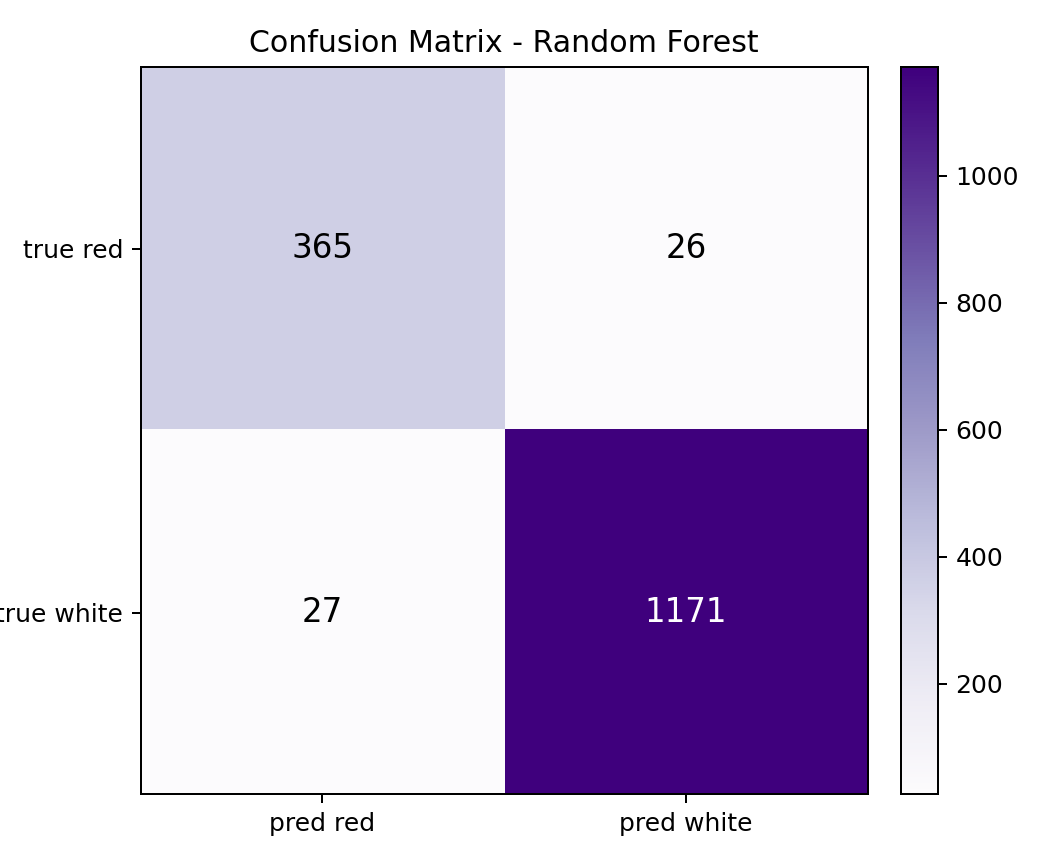
\includegraphics[width=0.62\textwidth]{q3_confusion_matrix.png}
\caption{Γραφική απεικόνιση του confusion matrix για το Random Forest.}
\end{figure}

\subsection{Πώς διαβάζουμε τον confusion matrix}

Ο confusion matrix μάς λέει:

\begin{itemize}
    \item 365 κόκκινα κρασιά ταξινομήθηκαν σωστά ως κόκκινα.
    \item 26 κόκκινα κρασιά ταξινομήθηκαν λάθος ως λευκά.
    \item 27 λευκά κρασιά ταξινομήθηκαν λάθος ως κόκκινα.
    \item 1171 λευκά κρασιά ταξινομήθηκαν σωστά ως λευκά.
\end{itemize}

Άρα οι σωστές προβλέψεις είναι:

\[
    365 + 1171 = 1536.
\]

Το συνολικό πλήθος test παρατηρήσεων είναι:

\[
    365 + 26 + 27 + 1171 = 1589.
\]

Επομένως:

\[
    \text{Accuracy} = \frac{1536}{1589} = 0.9666.
\]

Τα συνολικά λάθη είναι:

\[
    26 + 27 = 53.
\]

Άρα:

\[
    \text{Test Error} = \frac{53}{1589} = 0.0334.
\]

%=============================================================================
\section{Σύγκριση με τα προηγούμενα ερωτήματα}
%=============================================================================

Μέχρι τώρα έχουμε εφαρμόσει τρεις μεθόδους:

\begin{enumerate}[label=\arabic*.]
    \item Απλό δέντρο ταξινόμησης με \code{max\_depth=2}.
    \item Bagging με 200 δέντρα.
    \item Random Forest με 200 δέντρα και \code{max\_features=5}.
\end{enumerate}

Τα αποτελέσματα είναι:

\begin{table}[H]
\centering
\caption{Σύγκριση Ερωτημάτων 1, 2 και 3.}
\begin{tabular}{lrr}
\toprule
\textbf{Μοντέλο} & \textbf{Test Accuracy} & \textbf{Test Error} \\
\midrule
Decision Tree (\code{max\_depth=2}) & 0.9339 & 0.0661 \\
Bagging (200 estimators) & 0.9660 & 0.0340 \\
Random Forest (200 estimators, $m=5$) & 0.9666 & 0.0334 \\
\bottomrule
\end{tabular}
\end{table}

Σε σχέση με το απλό δέντρο, το Random Forest έχει πολύ καλύτερη απόδοση:

\[
    0.9666 - 0.9339 = 0.0327.
\]

Δηλαδή αυξάνει την ακρίβεια κατά περίπου 3.27 ποσοστιαίες μονάδες.

Σε σχέση με το Bagging, η διαφορά είναι μικρή:

\[
    0.9666 - 0.9660 = 0.0006.
\]

Άρα το Random Forest είναι ελαφρώς καλύτερο από το Bagging σε αυτό το test set,
αλλά η διαφορά είναι πολύ μικρή.

\subsection{Σύγκριση λαθών}

\begin{center}
\begin{tabular}{lrr}
\toprule
\textbf{Μοντέλο} & \textbf{Λάθη στο test set} & \textbf{Σωστές προβλέψεις} \\
\midrule
Decision Tree & 105 & 1484 \\
Bagging & 54 & 1535 \\
Random Forest & 53 & 1536 \\
\bottomrule
\end{tabular}
\end{center}

Το Random Forest έκανε ένα λάθος λιγότερο από το Bagging και 52 λάθη λιγότερα
από το απλό δέντρο.

%=============================================================================
\section{Σημαντικότητα χαρακτηριστικών}
%=============================================================================

Το Random Forest μπορεί να μας δώσει μία ένδειξη για το ποιες μεταβλητές
χρησιμοποιήθηκαν περισσότερο και βοήθησαν περισσότερο στους διαχωρισμούς των
δέντρων. Αυτό λέγεται \textbf{feature importance}.

\begin{figure}[H]
\centering
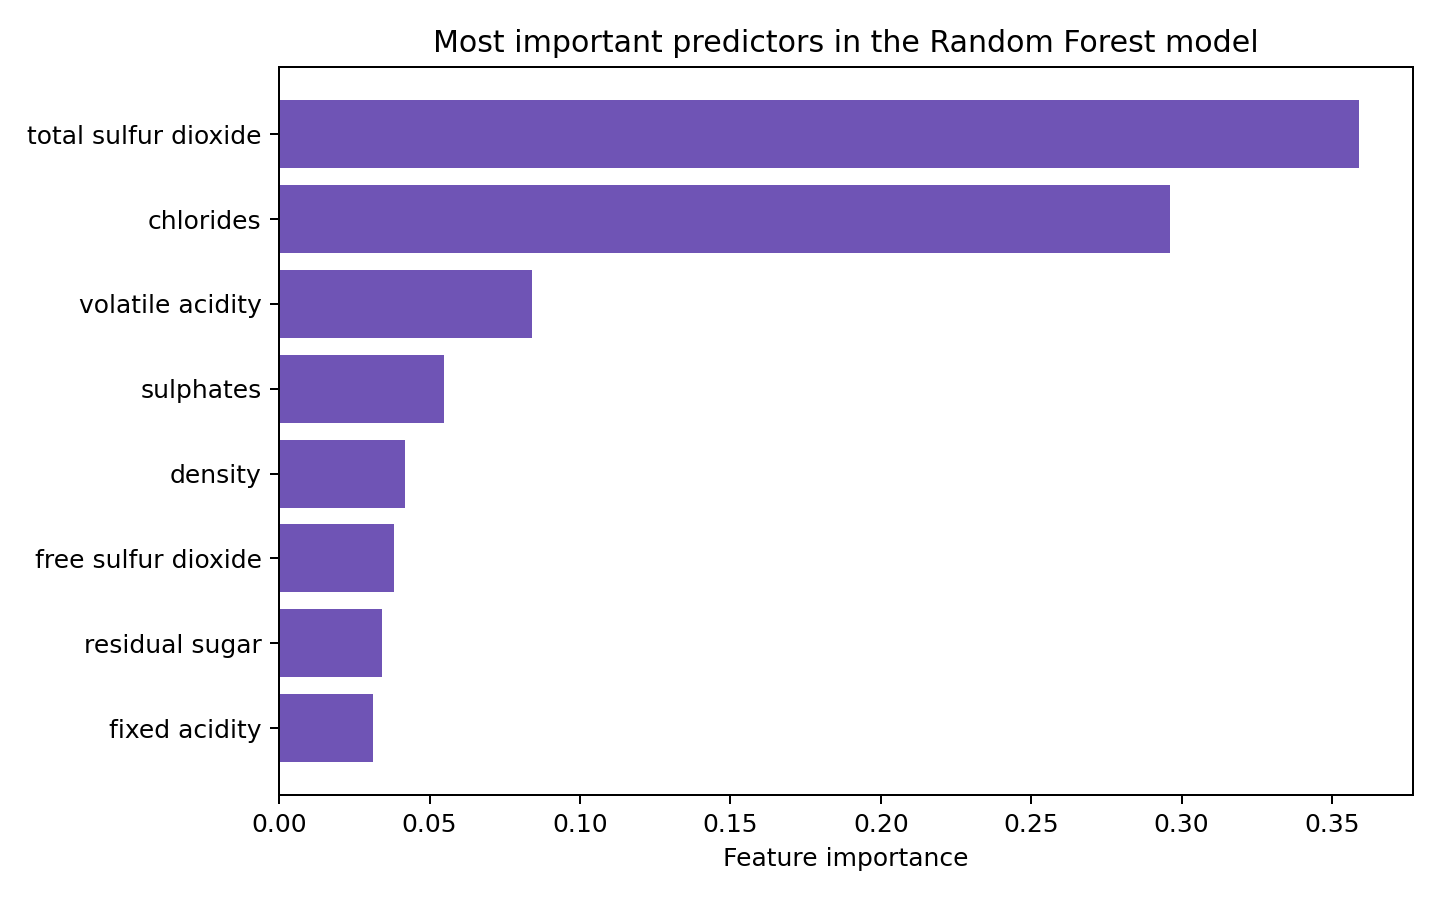
\includegraphics[width=0.82\textwidth]{q3_random_forest_feature_importance.png}
\caption{Οι σημαντικότερες μεταβλητές στο Random Forest.}
\end{figure}

\begin{table}[H]
\centering
\caption{Σημαντικότητα χαρακτηριστικών στο Random Forest.}
\small
\begin{tabular}{lr}
\toprule
\textbf{Μεταβλητή} & \textbf{Σημαντικότητα} \\
\midrule
\code{total sulfur dioxide} & 0.3590 \\
\code{chlorides} & 0.2962 \\
\code{volatile acidity} & 0.0842 \\
\code{sulphates} & 0.0547 \\
\code{density} & 0.0419 \\
\code{free sulfur dioxide} & 0.0381 \\
\code{residual sugar} & 0.0343 \\
\code{fixed acidity} & 0.0311 \\
\code{pH} & 0.0266 \\
\code{citric acid} & 0.0188 \\
\code{alcohol} & 0.0151 \\
\bottomrule
\end{tabular}
\end{table}

Παρατηρούμε ότι οι δύο σημαντικότερες μεταβλητές είναι:

\begin{itemize}
    \item \code{total sulfur dioxide}
    \item \code{chlorides}
\end{itemize}

Αυτό είναι συνεπές με όσα είδαμε στα προηγούμενα ερωτήματα. Το απλό δέντρο
του Ερωτήματος 1 βασίστηκε ακριβώς σε αυτές τις μεταβλητές. Το Bagging επίσης
τις ανέδειξε ως τις σημαντικότερες. Το Random Forest επιβεβαιώνει ότι τα
θειώδη και τα χλωριούχα άλατα είναι πολύ χρήσιμα για τη διάκριση λευκών και
κόκκινων κρασιών.

%=============================================================================
\section{Τελικός σχολιασμός για το Ερώτημα 3}
%=============================================================================

Το Random Forest με 200 δέντρα και \code{max\_features=5} πέτυχε test accuracy
0.9666. Αυτό είναι πολύ υψηλή ακρίβεια και δείχνει ότι η μέθοδος μπορεί να
προβλέψει με μεγάλη επιτυχία τον τύπο κρασιού.

Η απόδοση του Random Forest είναι πολύ καλύτερη από το απλό δέντρο του
Ερωτήματος 1 και ελαφρώς καλύτερη από το Bagging του Ερωτήματος 2. Η διαφορά
με το Bagging είναι μικρή, αλλά έχει νόημα: το Random Forest εισάγει επιπλέον
τυχαιότητα στην επιλογή χαρακτηριστικών, κάτι που μπορεί να μειώσει τη
συσχέτιση μεταξύ των δέντρων και να κάνει την τελική ψηφοφορία πιο αξιόπιστη.

Στο συγκεκριμένο dataset, το Random Forest έκανε 53 λάθη σε 1589 test
παρατηρήσεις. Αυτό σημαίνει ότι ταξινόμησε σωστά 1536 κρασιά. Οι περισσότερες
παρατηρήσεις ταξινομήθηκαν σωστά, ενώ τα λάθη ήταν σχετικά λίγα.

\subsection{Σύντομη απάντηση που μπορεί να μπει στην εργασία}

Για το τρίτο ερώτημα εφαρμόστηκε η μέθοδος Random Forest με
\code{n\_estimators=200}. Το πλήθος των προβλεπτικών μεταβλητών ήταν
$p=11$, άρα $p/2=5.5$. Επειδή το πλήθος υποψήφιων χαρακτηριστικών πρέπει να
δοθεί ως ακέραιος αριθμός, χρησιμοποιήθηκε \code{max\_features=5}. Το μοντέλο
εκπαιδεύτηκε στο training set και αξιολογήθηκε στο test set, με
\code{random\_state=6931}. Η test accuracy ήταν 0.9666 και το test error ήταν
0.0334. Ο confusion matrix έδειξε ότι ταξινομήθηκαν σωστά 365 κόκκινα και
1171 λευκά κρασιά, ενώ έγιναν συνολικά 53 λάθη. Το Random Forest είχε
ελαφρώς καλύτερη απόδοση από το Bagging και σαφώς καλύτερη από το απλό δέντρο
ταξινόμησης.

%=============================================================================
\appendix
\section{Αρχεία που δημιουργήθηκαν για το report}
%=============================================================================

Για το επεξηγηματικό report του Ερωτήματος 3 δημιουργήθηκαν τα παρακάτω
αρχεία:

\begin{itemize}
    \item \code{q3\_explanatory\_random\_forest.py}: script που αναπαράγει τη
    λύση.
    \item \code{q3\_explanatory\_results.csv}: συγκεντρωτικός πίνακας
    αποτελεσμάτων.
    \item \code{q3\_comparison\_q1\_q2\_q3.csv}: σύγκριση των τριών πρώτων
    μεθόδων.
    \item \code{q3\_confusion\_matrix.png}: εικόνα του confusion matrix.
    \item \code{q3\_random\_forest\_concept.png}: απλό σχήμα που εξηγεί τη
    μέθοδο Random Forest.
    \item \code{q3\_random\_forest\_feature\_importance.csv}: σημαντικότητα
    χαρακτηριστικών.
    \item \code{q3\_random\_forest\_feature\_importance.png}: γράφημα
    σημαντικότητας χαρακτηριστικών.
    \item \code{explanatory\_report\_q3\_random\_forest.tex}: το παρόν
    LaTeX αρχείο.
\end{itemize}

\end{document}
